% !TeX root = report.tex
% !TeX spellcheck = en_GB

\section{Results}
The results of the experiments can be seen on Figures \ref{experiments:graph:1}, \ref{experiments:graph:2}, \ref{experiments:graph:3} and \ref{experiments:graph:4}. The $x$ axis shows the generation, and the $y$ axis shows the champion fitness achieved for that generation in the run.

\begin{figure}[H]
	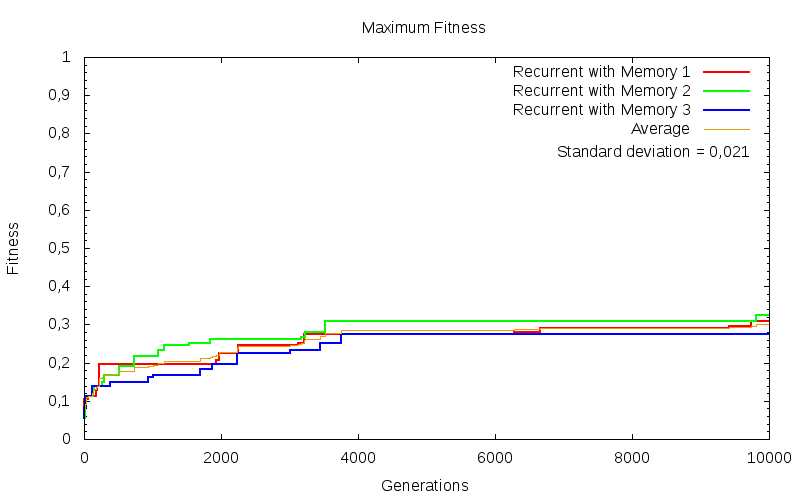
\includegraphics[width=\textwidth]{figures/recurrentmemory.png}
\caption{Graph of the results when using recurrent networks with enabled memory bank}
	\label{experiments:graph:1}
\end{figure}
\begin{figure}[H]
	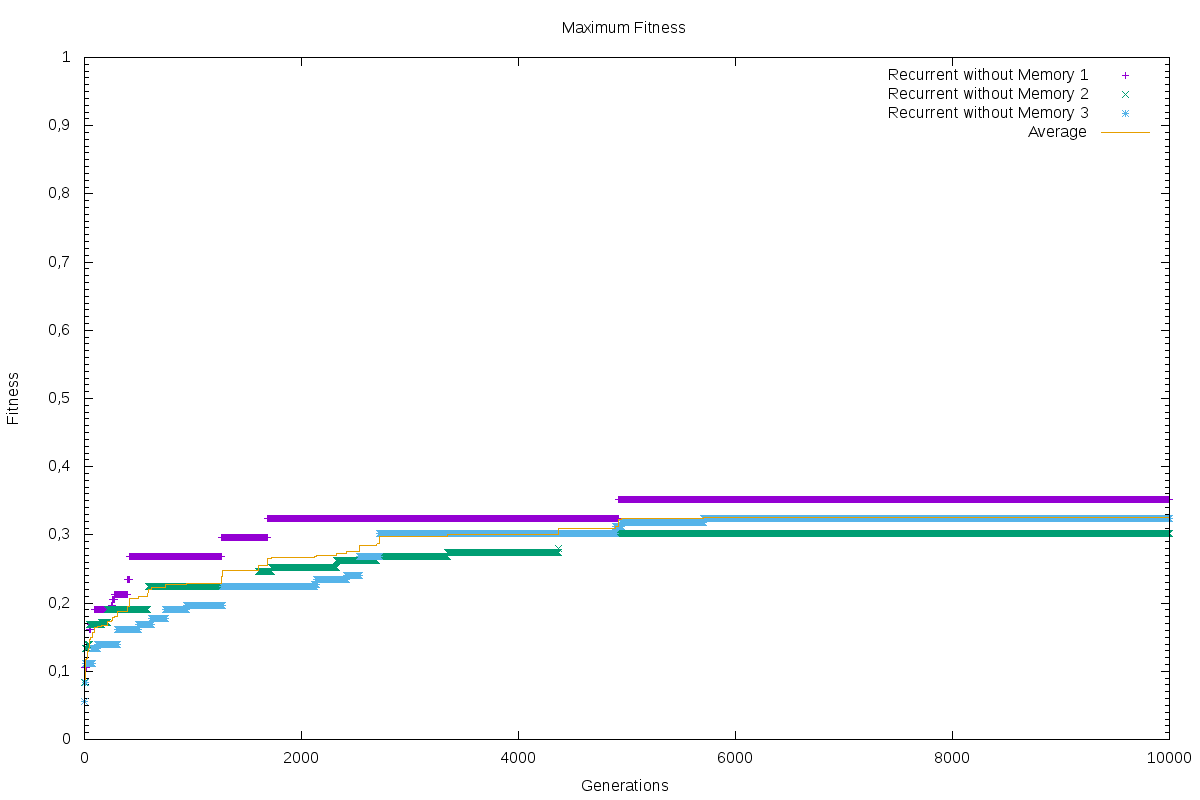
\includegraphics[width=\textwidth]{figures/recurrentnomemory.png}
	\caption{Graph of the results when using recurrent networks with disabled memory bank.}
		\label{experiments:graph:2}
\end{figure}

\begin{figure}[H]
	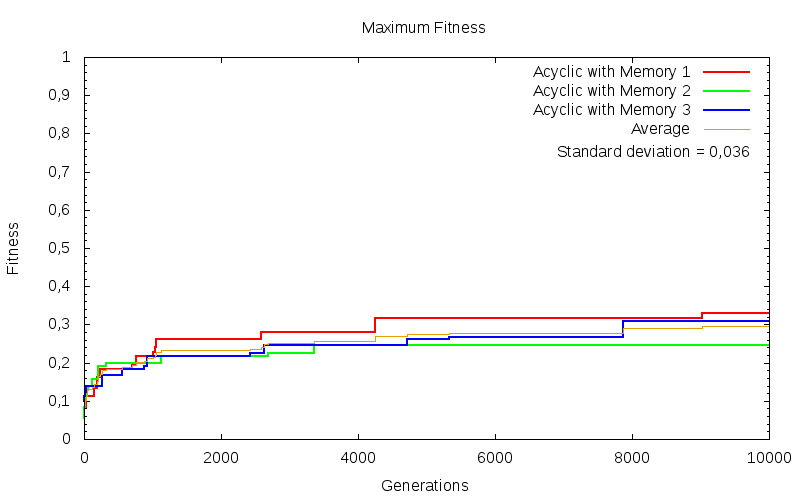
\includegraphics[width=\textwidth]{figures/acyclicmemory.png}
	\caption{Graph of the results when using acyclic networks with enabled memory bank.}
	\label{experiments:graph:3}
\end{figure}
\begin{figure}[H]
	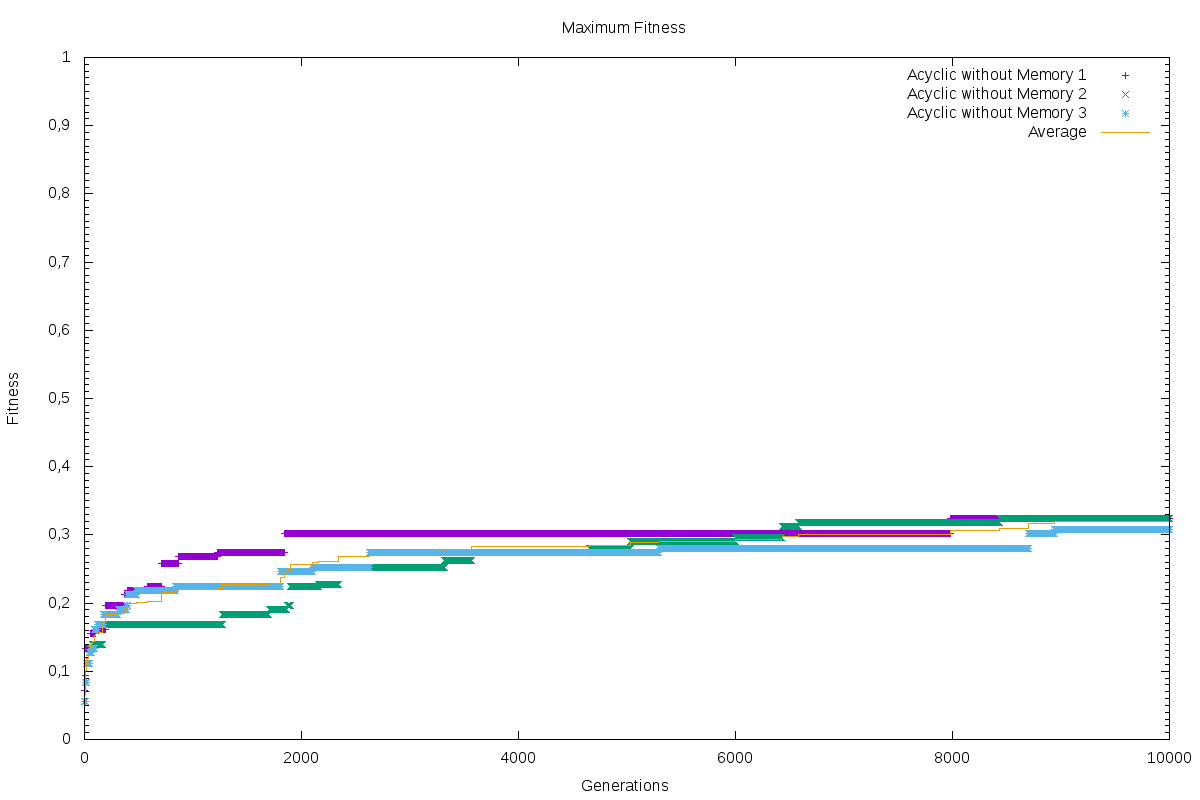
\includegraphics[width=\textwidth]{figures/acyclicnomemory.png}
	\caption{Graph of the results when using acyclic networks with disabled memory bank.}
	\label{experiments:graph:4}
\end{figure}

\begin{figure}[ht]
	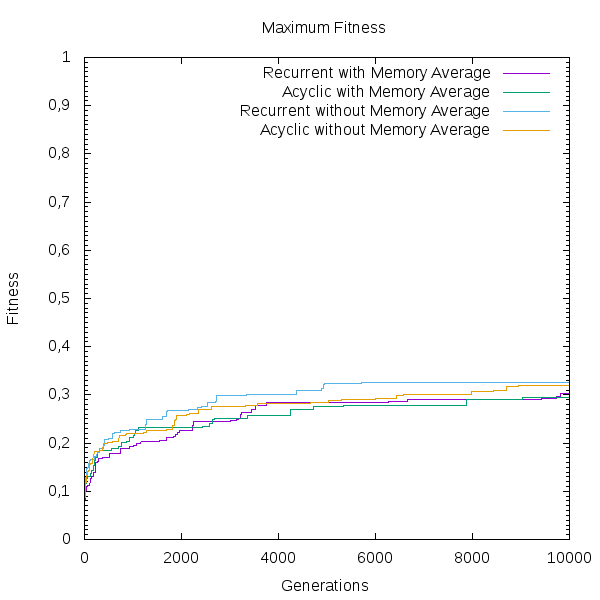
\includegraphics[width=\textwidth]{figures/averages.png}
	\caption{Averages over three runs of all configurations. Note that the y-axis has been truncated to make it easier to distinguish the different runs.}
	\label{experiments:graph:average}
\end{figure}

\newpar To compare the different experiments their averages are shown in \autoref{experiments:graph:average}. At generation 10.000 the averages show that both kinds of topologies find a better performing neural network when the Turing-functionality is turned off by a small margin of around 2\%.

\clearpage